\documentclass[11pt]{article}
\usepackage[margin=1in]{geometry}
\usepackage{amsmath, amssymb}
\usepackage{graphicx}
\usepackage{booktabs}
\usepackage{listings}
\usepackage{xcolor}
\usepackage{hyperref}
\usepackage{float}
\usepackage{animate}

\hypersetup{
    colorlinks=true,
    linkcolor=blue,
    urlcolor=blue
}

\begin{document}

% HEADER
\noindent
\textbf{Assignment 1} \\
\textbf{PHYS 142} \\
\textbf{Aman Palanati} \\
\textbf{TSN:} 200101723 \\
$x_{start} = \left(-1\right)^7\left(0.5 + \frac{23}{200}\right) = -0.615$ \\
\vspace{0.8em}
\hrule
\vspace{1.5em}

% BODY
\section*{Problem A:}
The $601 \times 601$ truncated matrix is:
\begin{center}
    \begin{verbatim}
    [[-0.05955846+0.0178667j  -0.0757611 +0.0217024j  -0.07967385+0.05414053j
      ... -0.46505982-0.30932634j -0.35439299-0.42735575j
      -0.21687407-0.50917202j]
     [-0.0757611 +0.0217024j  -0.0896081 +0.03330227j -0.08308486+0.06724787j
      ... -0.53404108-0.16837676j -0.46141968-0.31131639j
      -0.35439299-0.42735575j]
     [-0.07967385+0.05414053j -0.08308486+0.06724787j -0.06226964+0.09303051j
      ... -0.56407376-0.01040964j -0.53404108-0.16837676j
      -0.46505982-0.30932634j]
     ...
     [-0.46505982-0.30932634j -0.53404108-0.16837676j -0.56407376-0.01040964j
      ... -0.06226964+0.09303051j -0.08308486+0.06724787j
      -0.07967385+0.05414053j]
     [-0.35439299-0.42735575j -0.46141968-0.31131639j -0.53404108-0.16837676j
      ... -0.08308486+0.06724787j -0.0896081 +0.03330227j
      -0.0757611 +0.0217024j ]
     [-0.21687407-0.50917202j -0.35439299-0.42735575j -0.46505982-0.30932634j
      ... -0.07967385+0.05414053j -0.0757611 +0.0217024j
      -0.05955846+0.0178667j ]]
    \end{verbatim}
\end{center}

\section*{Problem B:}
\begin{figure}[H]
  \centering
  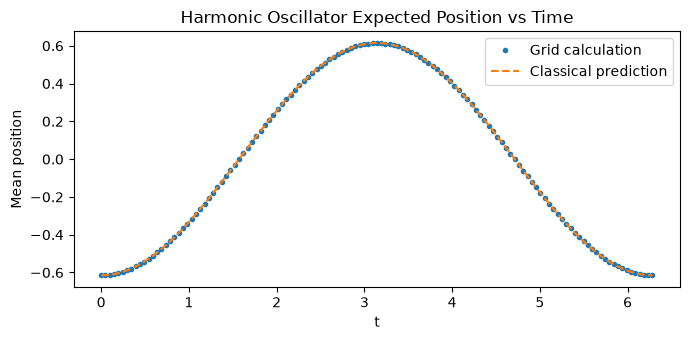
\includegraphics[width=0.9\textwidth]{problemB.png}
\end{figure}

\section*{Problem C:}
\begin{figure}[H]
  \centering
  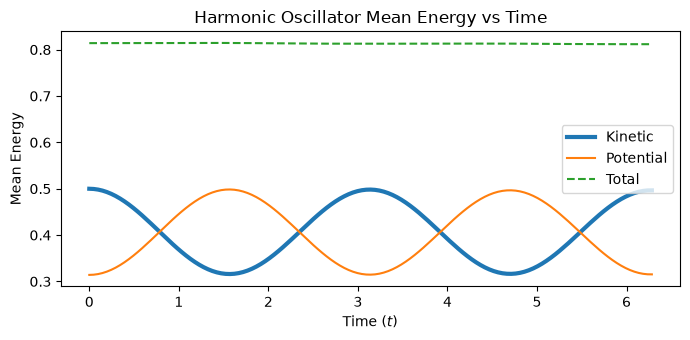
\includegraphics[width=0.9\textwidth]{problemC.png}
\end{figure}

\section*{Problem D:}
\begin{figure}[H]
  \centering
  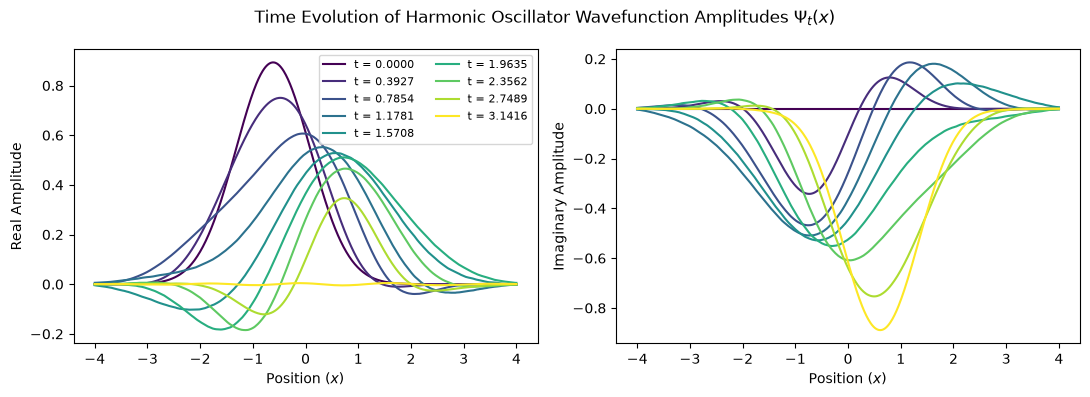
\includegraphics[width=0.9\textwidth]{problemD.png}
\end{figure}

\section*{Problem E:}
\begin{figure}[htbp]
    \centering
    % Arguments: controls, autoplay, loop, fps, path template, start index, end index
    \animategraphics[controls,autoplay,loop,width=0.95\textwidth]{15}{frames/frame_}{000}{128}
\end{figure}
\setlength{\parindent}{0pt} The animated time evolution of the harmonic oscillator wavefunction over one full period is shown in the separately submitted problemE.gif.

\section*{Problem F:}
\textbf{Prediction:} Since $\epsilon$ is extremely small, so the phase of $\mathcal{K}_{\epsilon}$ can be approximated as $\phi \approx \frac{\left(x_b - x_a\right)^2}{2\epsilon}$. Using a Riemann approximation for the phase change between time steps, this becomes $\Delta\phi \approx \frac{\left(x_b - x_a\right)\cdot\Delta x}{\epsilon}$. If $\Delta \phi$ is too large, destructive interference fails, so $\mathcal{N}(t)$ diverges which causes the total probability to blow up. The largest possible separation between two points is 8, so we get:\\
\vspace{-1.5em}
\begin{center}
Case (i): $\Delta \phi \approx 0.271$ rad \\
Case (ii): $\Delta \phi \approx 8.69$ rad \\ 
Case (iii): $\Delta \phi \approx 8.69$ rad \\
\end{center}
Therefore, Cases (ii) and (iii) will fail because the calculated $\Delta \phi$ is very large.

\begin{figure}[H]
  \centering
  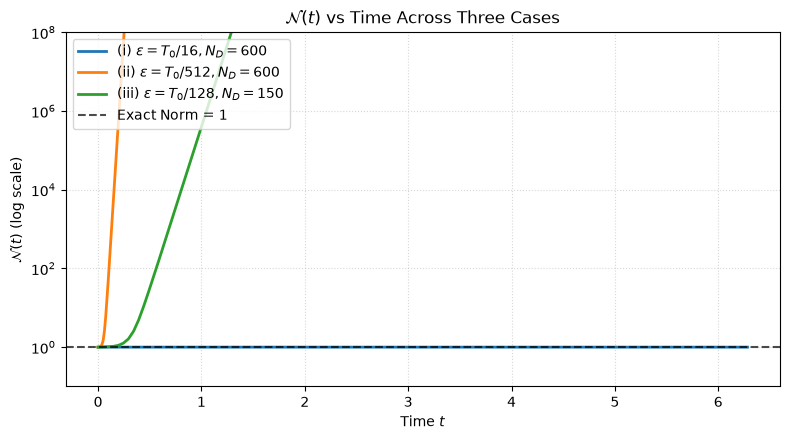
\includegraphics[width=0.9\textwidth]{problemF.png}
\end{figure}

\setlength{\parindent}{0pt} In Case (i), a large $\epsilon$ causes $\mathcal{K}_\epsilon(x_b, x_a)$ to oscillate slowly across $x_a$, allowing the grid spacing $\Delta x$ with $N_D = 600$ to preserve $\mathcal{N} = 1$. In Case (ii), a small $\epsilon$ causes $\mathcal{K}_\epsilon$ to oscillate too quickly for $\Delta x$ to capture, while in Case (iii), making the grid spacing larger with $N_D = 150$ makes $\Delta x$ too large to capture the oscillations. In both Cases (ii) and (iii), the phase change between neighboring grid points is very large, so destructive interference fails, causing the norm to diverge exponentially. \\
Using the Nyquist sampling rate as an approximation, the phase change between neighboring grid points cannot be greater than $\pi$, so $\Delta \phi \approx \frac{8 \Delta x}{\epsilon} \le \pi$.
   $$\epsilon_{\min} \approx \frac{8 \Delta x}{\pi} \approx \frac{8 \times (8 / 600)}{\pi} \approx 0.0340 \approx \frac{T_0}{185}$$
$\epsilon_{\min}$ scales linearly $\Delta x$, and doubling $N_D$ to $2N_D$ cuts $\Delta x$ in half, so the minimum timestep is halved as well: $\epsilon_{\min} \approx 0.0170 \approx \frac{T_0}{370}$

\section*{AI Use Appendix:}

\begin{enumerate}
    \item \textbf{Tools and Usage:} Google Gemini was used for writing/debugging Python code, obtaining conceptual explanations for each of the problems, structuring the report, and final verification of submissions.

    \item \textbf{Prompts:} My prompts were focused on getting implementations and explanations and troubleshooting: calculating $x_{\text{start}}$ from TSN, explanations for outer-product calculation of $\mathcal{K}_\epsilon$, setting up energy expectation values, exporting GIF animations via \texttt{FuncAnimation}, predicting and explaining the $\Delta \phi > \pi$ limit in Problem F, and resolving Python \texttt{TypeError} and LaTeX compiler errors. Full chat transcript: \url{https://share.gemini.google/jH5WUwbDI8N2}.
    
    \item \textbf{Errors and Verification:} 
    \begin{itemize}
        \item \textit{Variable Inconsistency:} In Problem F the model initially reused static $\sin(\omega \epsilon)$ and $\cos(\omega \epsilon)$ variables from standard $\epsilon$ instead of recomputing them for $\Delta t_{\text{case}}$. This was caught by inspecting output energy plots against conservation of energy and checking norm divergence curves to ensure they matched what I expected.
        \item \textit{JSON Formatting:} The model omitted quotation marks around dictionary keys (\texttt{tsn} and \texttt{x\_start}) during export, causing a \texttt{TypeError}. Caught during notebook cell execution.
        \item \textit{LaTeX Syntax:} A runaway argument syntax error was generated due to an unclosed \texttt{\textbackslash textbf} tag. Caught via Overleaf compiler crash logs and corrected before final compilation.
    \end{itemize}
\end{enumerate}

\end{document}